\section{Lec 22}
\subsection{Gravitational waves - Traceless gauge}
We want to study propagating degrees of freedom of the gravitational field, which require no local source to exist. So we will use weak field equations in transverse gauge, but keeping time derivatives and shutting off $T_{\mu \nu }$, setting it at zero.\par
Then $G_{00} = 0 $ and $\nabla^{2}\Psi  = 0$, and since this has to be well behaved, $\Psi =0$.\par

Same story for $G_{0i} = 0 $ equation, gives $-\nabla ^{2}w_{i} =0$ and for same reasons $w_{i} = 0$.\par
Trace of $G_{ij} $ gives $\nabla ^{2}\phi =0$ and so $\phi =0$.\par
Traceless $G_{ij}$ leaves $\Box s_{ij} = 0$, that is a wave equation for $s_{ij}$. We have all degrees of freedom of $h_{\mu \nu }$ are set to zero except for $s_{ij}$ (that is transverse), and we express this setup with the \emph{transverse traceless gauge}
\[
h_{\mu \nu }^{TT} = \begin{pmatrix}
0 & 0 & 0 & 0 \\
0 & 2s_{11} & 2s_{12} & 2s_{13} \\
0 & 2s_{21} & 2s_{22} & 2s_{23} \\
0 & 2s_{31} & 2s_{32} & 2s_{33}
\end{pmatrix} 
\]
And the equation of motion is 
\[
\Box h_{\mu \nu }^{TT} =0
\]
There are some properties of this tensor
\begin{align}
h_{0 \nu }^{TT} = 0 =  h^{TT}_{\nu 0} \\
\eta ^{\mu \nu } h^{TT}_{\mu \nu } =0\\
\partial_{\mu }h^{TT}_{\mu \nu } = 0
\end{align}

We want to look for some solution of this equation of motion, and they could be the plane waves
\[
h^{TT}_{\mu \nu } = C_{\mu \nu }e^{ik_{\sigma x^{\sigma }}}
\]
where $C_{\mu \nu }$ is made of constants $\in \mathbb{R}$, while the exponential $\in \mathbb{I}$, but we will keep the \emph{real part}, so that the tensor on the left $\in \mathbb{R}$.\par

We can try to plug this inside the equation of motion
\begin{align*}
	0 &= \Box h^{TT}_{\mu \nu }\\
	  &= \eta ^{\alpha \beta }\partial_{\alpha }\partial_{\beta }\left( C_{\mu \nu }e^{ik_{\sigma }x^{\sigma }} \right) \\
	  &= - \left( \eta ^{\alpha \beta }k_{\alpha }k_{\beta }h^{TT}_{\mu \nu } \right)\\
	  &= k_{\alpha }k^{\alpha }
\end{align*}
so that last product is equal to zero. We know that $k^{\mu } =\left( \omega , k^{1},k^{2},k^{3} \right)$, it's a wave vector, and if this vector is null, it solves the equation of motion, that could be loosely translated into "the GW propagate at speed of light".\par
To have wave vector null, we need that
\[
k^{\alpha }k_{\alpha } = 0 \to - \omega ^{2} + \vec{k}\cdot \vec{k}=0
\]
Now we need to ensure that the perturbation is transverse, we can have a kinda explicit solution by choosing spatial coordinates such that the wave is travelling along the \emph{z axis.}\par
So
\begin{align*}
k^{\sigma } = \left( \omega , 0,0, \omega  \right)\\
h^{TT}_{\mu \nu } = C_{\mu \nu }e^{i\left( -\omega t +\omega z \right)} 
\end{align*}
and by taking the real part we get
\[
h^{TT}_{\mu \nu } = C_{\mu \nu } \text{cos}\left( \omega \left( t-z \right) \right)
\]
that is the solution for a wave-front propagating at \emph{c}.\par
We would like to add some information about $C_{\mu \nu }$. It is a constant, symmetric tensor, which is traceless and purely spatial. So it fills the $i,j$ region of the $h_{\mu \nu }^{TT}$, with $i\neq j$
\begin{gather*}
C_{0\nu } = 0 = C_{\nu 0} \\
\eta ^{\mu \nu }C_{\mu \nu } = 0
\end{gather*}

With this particular solution of the traceless transverse gauge, since 
\[
\partial_{\mu }h^{TT}_{\mu \nu } = 0 \to k_{\mu }C^{\mu \nu } = 0
\]
this means that the wave vector is orthogonal to $C^{\mu \nu }$. This can be expanded such that 
\[
k^{0}G_{0\nu } + k^{3}C_{3\nu } = 0 \to  C_{3\nu } = 0 = C_{\nu  3}
\]
and this implies that $C_{\mu \nu }$ fills only the $i,j = 1,2$ region of $h^{TT}_{\mu \nu }$ such that
\[
C_{\mu \nu } = \begin{pmatrix}
0 & 0 & 0 & 0 \\
0 & C & C & 0 \\
0 & C & C & 0 \\
0 & 0 & 0 & 0
\end{pmatrix} = \begin{pmatrix}
0 & 0 & 0 & 0 \\
0 & h_{+} & h_{\times} & 0 \\
0 & h{\times} & h_{+} & 0 \\
0 & 0 & 0 & 0
\end{pmatrix} 
\]
Since it is traceless $C_{11} = -C_{22}$, and symmetric $C_{12} = C_{21}$.\par
For a plane wave in this gauge travelling in \emph{z} direction, two components $C_{11}, C_{12}$, with $\omega $, characterize the wave.

We will redefine $C_{\mu \nu }$ components such that
\[
h_{\mu \nu  }^{TT}= \begin{pmatrix}
0 & 0 & 0 & 0 \\
0 & h_{+} & h_{\times} & 0 \\
0 & h_{\times} & -h_{+} & 0 \\
0 & 0 & 0 & 0
\end{pmatrix} e^{i \omega \left( t-z \right)}
\]
Then one could ask, why $+, \times$ ? \par
To answer this question it's useful to get out hands on a tangible phenomenon. Let's take the motion of a test particle in presence of a wave. 
\[
\frac{d u^{\alpha }}{d \tau } + \Gamma ^{\alpha }_{\mu \nu }u^{\mu }u^{\nu }
\]
at $t=0 \to u^{\alpha }= \left( 1,0,0,0 \right)$, and so
\[
 \left.\frac{d u^{\alpha }}{d \tau }\right|_{t=0} = - \Gamma ^{\alpha }_{00} = -\frac{1}{2}\eta ^{\alpha \beta }\left( 2\partial_{0}h_{\beta 0}-\partial_{\beta h_{00}} \right) =0
\]
but we see that GW have not effect on test particle.\par

To obtain a coordinate independent measure of the effects of GW, we consider the relative motion of two test particles, set like this\par
\bigskip
\begin{center}
\begin{tikzpicture}[x=0.60pt,y=0.60pt,yscale=-1,xscale=1]
\draw    (292.67,230.25) -- (291.68,36.25) ;
\draw [shift={(291.67,34.25)}, rotate = 89.71] [color={rgb, 255:red, 0; green, 0; blue, 0 }  ][line width=0.75]    (10.93,-3.29) .. controls (6.95,-1.4) and (3.31,-0.3) .. (0,0) .. controls (3.31,0.3) and (6.95,1.4) .. (10.93,3.29)   ;
\draw    (292.67,230.25) -- (458.67,230.25) ;
\draw [shift={(460.67,230.25)}, rotate = 180] [color={rgb, 255:red, 0; green, 0; blue, 0 }  ][line width=0.75]    (10.93,-3.29) .. controls (6.95,-1.4) and (3.31,-0.3) .. (0,0) .. controls (3.31,0.3) and (6.95,1.4) .. (10.93,3.29)   ;
\draw  [fill={rgb, 255:red, 0; green, 0; blue, 0 }  ,fill opacity=1 ] (418,231.13) .. controls (418,228.98) and (419.73,227.25) .. (421.88,227.25) .. controls (424.02,227.25) and (425.75,228.98) .. (425.75,231.13) .. controls (425.75,233.27) and (424.02,235) .. (421.88,235) .. controls (419.73,235) and (418,233.27) .. (418,231.13) -- cycle ;
\draw  [fill={rgb, 255:red, 0; green, 0; blue, 0 }  ,fill opacity=1 ] (288.79,234.13) .. controls (288.79,231.98) and (290.53,230.25) .. (292.67,230.25) .. controls (294.81,230.25) and (296.54,231.98) .. (296.54,234.13) .. controls (296.54,236.27) and (294.81,238) .. (292.67,238) .. controls (290.53,238) and (288.79,236.27) .. (288.79,234.13) -- cycle ;
\draw  [fill={rgb, 255:red, 0; green, 0; blue, 0 }  ,fill opacity=1 ] (289,91.13) .. controls (289,88.98) and (290.73,87.25) .. (292.88,87.25) .. controls (295.02,87.25) and (296.75,88.98) .. (296.75,91.13) .. controls (296.75,93.27) and (295.02,95) .. (292.88,95) .. controls (290.73,95) and (289,93.27) .. (289,91.13) -- cycle ;
\draw (259,235) node [anchor=north west][inner sep=0.75pt]   [align=left] {A};
\draw (416,249) node [anchor=north west][inner sep=0.75pt]   [align=left] {B};
\draw (243,77) node [anchor=north west][inner sep=0.75pt]   [align=left] {C};
\draw (315.95,213.84) node [anchor=north west][inner sep=0.75pt]  [font=\Huge,rotate=-270.38] [align=left] {\}};
\draw (331,171) node [anchor=north west][inner sep=0.75pt]   [align=left] {$\delta$};
\draw (476,230) node [anchor=north west][inner sep=0.75pt]   [align=left] {x};
\draw (259,29) node [anchor=north west][inner sep=0.75pt]   [align=left] {y};
\end{tikzpicture}
\end{center}\par
\bigskip
We see that at $t=0, D_{AB} = \delta $, and after GW
\[
D_{AB} = \int_{A}^{B}{\sqrt{g_{11}}dx} = \int_{A}^{B}{\sqrt{1+h_{11}}dx}\approx \left( 1 + \frac{h_{+}}{2} \right)\delta 
\]
while the \emph{vertical} distance
\[
D_{AC} \approx \left( 1+ \frac{h_{22}}{2} \right)\delta = \left( 1 - \frac{h_{+}}2{} \right)\delta  
\]
we see that the effects are the opposites. In fact the outcome would be something like

\begin{figure}[h]
\centering
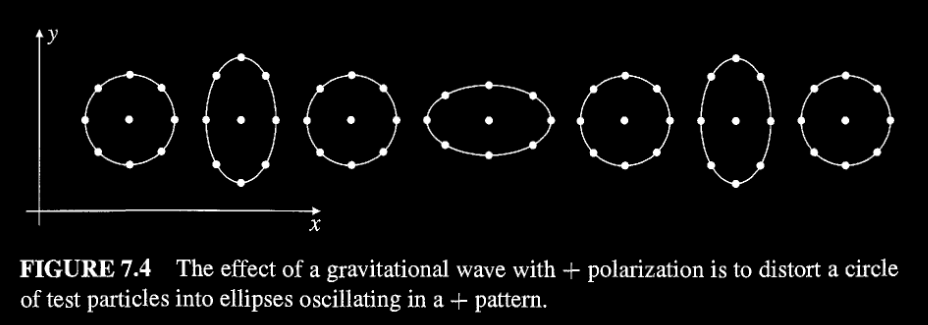
\includegraphics[width=\linewidth]{imm/gweffect.png}
\caption{effect of GW}
\label{imm:gweffect.png}
\end{figure}


















